% !TEX encoding = UTF-8 Unicode
\documentclass[a4paper]{article}

\usepackage{url}
\usepackage{xcolor}
\usepackage{graphicx}
\graphicspath{{../Slike/}}
\usepackage[english,serbianc]{babel}
\usepackage[unicode]{hyperref}
\hypersetup{colorlinks,
                   citecolor=gray,
                   filecolor=gray,
                   linkcolor=blue,
                   urlcolor=blue}

% Овако фонт неће бити блед тј. инсталираће
% се квалитетни фонтови за случај да већ нису
\usepackage{type1ec}

% Овако је могуће претраживати и копирати ћирилицу
% из генерисаног документа, независно од хифенације
\usepackage{cmap}
\defaulthyphenchar=127

% Овако је могуће имати нпр. опис нечега у два реда
\newcommand{\dvareda}[2][c]{\begin{tabular}[#1]{@{}c@{}}#2\end{tabular}}

\begin{document}

\title{Минимално многоугаоно раздвајање два скупа тачака у равни}

\author{Лазар Васовић}

\date{15. април 2020.}

\maketitle

\abstract{Размотрен је проблем проналаска најмањег (у смислу обима) многоугла који раздваја два коначна скупа црвених и плавих тачака у равни. Циљни полигон, чија су темена из тих скупова и чија се боја занемарује, дели раван на два дела -- унутрашњост и спољашњост -- тако да су све тачке које се налазе у једном делу исте боје, док се боја тачака у различитим деловима разликује. Изложен је контролни алгоритам исцрпне претраге који проналази оптимум, а затим и нека хеуристичка решења из литературе, случајна и локална претрага. На крају је предложена еволутивна метахеуристика заснована на генетском алгоритму, као и оптимизација јатом птица из групе интелигенције ројева -- обе успешно хибридизоване са симулираним каљењем.}

\tableofcontents

\newpage

\section{Уводна реч}

\textbf{Проблеми раздвојивости} су распрострањени у разним сферама живота и постоје у много облика. Како само име сугерише, задатак је на неки начин раздвојити два или више скупова објеката. Познат је проблем раздвојивости два коначна скупа тачака, од којих се један означава као скуп \textbf{црвених}, а други као скуп \textbf{плавих тачака} (отуд енгл. \textit{red-blue separability}). Како су у питању тачке неког простора, овај задатак припада групи проблема \textbf{геометријске раздвојивости}. 

Међу најпознатијима је проблем \textbf{линеарне сепарабилности} два скупа тачака у еуклидској равни, у коме се поставља питање постоји ли права таква да се са њене једне стране налазе искључиво црвене, а са друге искључиво плаве тачке. Уобичајени захтев је и да та права не садржи тачке из скупова, како би раздвајање било потпуно, без тачака на граници. Уколико се уз потврдан одговор захтева и сама права односно њена једначина, опциони захтев је да је маргина максимална односно да је растојање између тачака најближих раздвајајућој правој што веће, чиме се постиже боља подела простора. Ово указује на везу између проблема раздвојивости и \textbf{просторног партиционисања}.

Напреднија верзија проблема јесте проблем \textbf{нелинеарне сепарабилности}, који се може решити на два основна начина. Први је карактеристичан за метод потпорних вектора (SVM) и састоји се из испитивања линеарне сепарабилности над трансформисаним тачкама. Међутим, у том случају није лако могуће у полазном простору наћи \textbf{раздвајајућу структуру} која би одговарала добијеној правој у трансформисаном. Као решење тога намећу се алгоритми који испитују раздвојивост без икаквих измена улазних података. Управо су они тема овог рада, при чему се за раздвајајућу структуру узимају \textbf{прости многоуглови}. Поред њих, могуће је радити са скуповима правих (нпр. \cite{bonnet}), круговима (нпр. \cite{cheung}) или неким другим структурама, што је одлика новијих радова.

Како је напоменуто, проблем раздвојивости једнак је проблему поделе простора. Наиме, свака раздвајајућа структура на неки начин дели раван на потпростор(е) са само црвеним и потпростор(е) са само плавим тачкама. У складу са тим, питање је колико се потпростора на крају добије. У овом раду фокус је на поделу \textbf{тачно једним} простим многоуглом, тако да ће подела бити на тачно \textit{два потпростора} -- унутрашњост и спољашњост -- таква да су тачке које се налазе у једном исте боје, док је боја тачака у различитим деловима различита.

Када је раздвајајућа структура фиксирана на прост многоугао, отворено је питање његових темена. Добар део разматрања допушта да темена буду произвољне тачке простора, међу којима се издвајају \cite{mitch}, \cite{mata}, \cite{arora}, као и \cite{gud}. Њихова дељена идеја заснована је на рекурзивној подели простора док се не дође до делова који садрже тачке само једне боје, а затим спајање тих делова у један. Решење је полигон који чини границе добијених делова. Још једна могућа идеја у овом случају било би генерисање Воронојевог дијаграма, који прецизно дели простор на делове који припадају свакој тачки појединачно, а затим спајање  резултујућих ћелија према боји. Ипак, у овом раду је \textbf{избор темена фиксиран} на задати скуп тачака, као што је у \cite{eades} или \cite{edels}, како би домен био коначан. Разматрају се само многоуглови са свим темена из скупа црвених и плавих тачака, чија се боја \textit{занемарује}.

Након што су дефинисани основа проблема и допустива решења, неопходно је дефинисати и циљ, како би оптимизациони проблем био комплетиран. У конкретом случају, тражи се минимално полигонално раздвајање, тако да ће се \textbf{минимизовати обим} допустивих многоуглова. Како није могуће наћи тачно решење без испитивања целокупног скупа могућих решења, верзија овог проблема са одлучивошћу -- постоји ли раздвајајући полигон обима мањег од $k$ -- припада групи \textbf{NP-тешких} проблема. Доказ те тврдње свођењем проблема трговачког путника на овај дат је у \cite{eades}.

Сваки оптимизациони проблем над коначним доменом, па и овај, могуће је решити \textbf{егзактно}, провером сваког члана домена. Ипак, тежина условљава експоненцијално време извршавања таквог алгоритма, што овакво решавање чини практично неупотребљивим за иоле већу димензију улаза. Из тог разлога се прибегава употреби \textbf{хеуристика}, које дају приближно решење, али се извршавају у полиномском времену. Један од проблема оваквог решавања је специфичност, пошто једном осмишљена хеуристика често није поново употребљива, осим за неке веома сличне проблеме. Стога се за потребе наглашавања употребљивости на широком спектру оптимизационих проблема уводи појам \textbf{метахеуристике}. Метахеуристичке методе описују опште стратегије претраге за решавање оптимизационих проблема. Формулисане су независно од конкретног проблема, али су прилагодљиве посебном проблему који се решава. У раду су примењене све три стратегије, при чему прве две служе за контролу трећег приступа.

\section{Контролни алгоритми}

Приликом решавања проблема који су фактички већ решени, паметно је своје решење упоредити са претходним, доступним у литератури. Те већ осмишљене методе могу се означити као \textbf{контролни алгоритми}. Чак и у случају да се решава нов проблем, увек је за оне засноване на претрази коначног домена могуће осмислити алгоритам који у експоненцијалном времену претражује целокупан домен.

\subsection{Исцрпна претрага}

Најједноставнији алгоритам за решавање проблема претраге јесте \textbf{исцрпна претрага} односно \textbf{тотална енумерација}. У питању је \textit{метод грубе силе} који просто провери свако потенцијално решење из домена и тако нађе оно најбоље. Како не постоји посебна правилност у идеји потпуног набрајања, у питању је \textit{неусмерена претрага}. Најважнија одлика овог приступа јесте \textbf{оптималност} односно \textit{егзактност} односно \textit{гаранција} да је пронађено решење најбоље могуће тј. тачно.

Међутим, невоља код тешких проблема је њихова експоненцијална природа, тако да би, у конкретном случају са два скупа тачака, већ за двадесетак тачака проста исцрпна претрага морала да провери преко два трилиона ($20! > 2\cdot10^{18}$) потенцијалних решења. Овај број је могуће вишеструко умањити прецизнијом анализом проблема. Наиме, уколико постоји $n$ тачака, у обзир долазе сви многоуглови од троугла до $n$-тоугла. За сваки од њих тј. за свако $k \in \{3..n\}$ могуће је одабрати ${n \choose k}$ различитих $k$-торки тачака, док је од сваке $k$-торке могуће формирати $(k-1)!/2$ различитих мада не нужно простих $k$-гона. Дакле, иако постоји увећање димензије због параметра $k$, знатно умањење доноси разматрање само различитих полигона (нпр. троугао $ABC$ исти је као $BCA$ или $CBA$) уместо свих $k!$ пермутација тачака. Ово доводи до укупног броја од $\frac{1}{2} \sum_{k=3}^{n} {n \choose k} (k-1)!$, што је око четрнаест пута мање од само $n!$ за $n = 20$. Управо ова сума узета је за основу имплементације за проучавани проблем. Наравно, услед његове неефикасности, овај метод примењен је само на мале тест примере, углавном у сврхе анализе самог проблема и контроле успешности даљих стратегија.

Пре имплементације, неопходно је још одредити \textbf{кодирање решења}, као и \textbf{функцију прилагођености} која ће послужити као мера квалитета решења. Како је у питању \textit{пермутациони проблем}, кодирање се лако решава као низ тачака. Примера ради, уколико је решење троугао који, тим редом, чине тачке 3, 7, 13 одговарајући код је $[3, 7, 13]$. Функција прилагођености мало је компликованија. Прво је неопходно одредити обим полигона, што би у случају троугла $[3, 7, 13]$ био збир дужина дужи $3|7$, $7|13$ и $13|3$. Други корак је одређивање допустивости. Уколико решење не раздваја добро простор, бива кажњено тако што му се дужина множи минималним бројем тачака које се налазе у погрешном потпростору. Недопустивост настала зато што добијени многоугао није прост кажњава се десетоструко.

Имплементација јединке (решења) налази се у датотеци \textit{jedinka.py}, а заснована је на библиотеци \textit{Shapely}, која омогућава комфорно израчунавање обима, припадности и валидности. Јединка наслеђује уграђену класу за многоугао, а функционалности проширује чувањем расподеле тачака, броја промашаја, кода јединке и скора односно прилагођености израчунате према опису. Сама минимизација по претходно описаном скупу могућих решења одрађена је у фајлу \textit{algoritmi.py}. Омогућено је читање података из датотеке која садржи листу тачака и одговарајућих боја. Најпростији представљен тест пример је у фајлу \textit{ulaz9.txt} и има девет тачака. Егзактно решење дато је на слици \ref{iscrpna9}.

\begin{figure}[h!]
\begin{center}
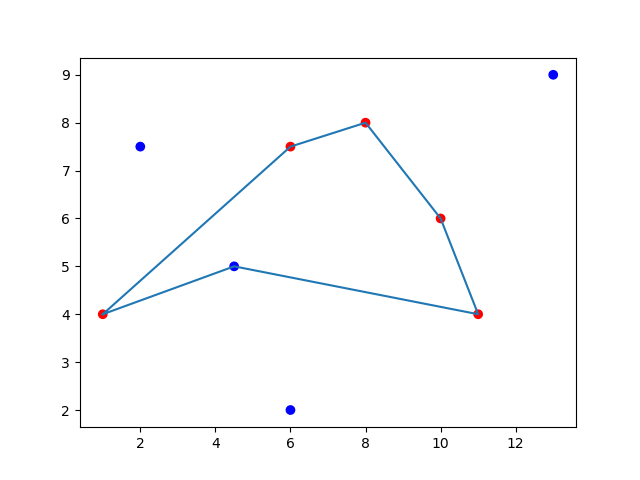
\includegraphics[scale=0.64]{iscrpna9.png}
\end{center}
\caption{Тачно решење тест примера \textit{ulaz9.txt}}
\label{iscrpna9}
\end{figure}

Решење је допустиво пошто је полигон прост и дели раван у складу са захтевима. Његов код је $[0, 2, 7, 6, 5, 3]$, а обим и скор 23,45. Нема промашених тачака, темена су пет црвених и једна плава тачка, спољашњост садржи само плаве тачке, а унутрашњост је празна.

Алгоритам исцрпне претраге искоришћен је и у сврхе емпиријске анализе самог проблема. Важан податак је колики део потенцијалних решења је допустив, као и колико су допустива решења у просеку блиска тачном. За те потребе су помоћу скрипта \textit{histogram.py} прикупљени сви скорови у датотеку \textit{skor9.txt}. Испоставља се да је тек свако педесето решење допустиво, као и да допустива махом нису блиска, али се чини да имају нормалну расподелу са средином око 40. Све ово представљено је на хистограму на слици \ref{hist9}, као и у табели \ref{udeo9}.

\begin{figure}[h!]
\begin{center}
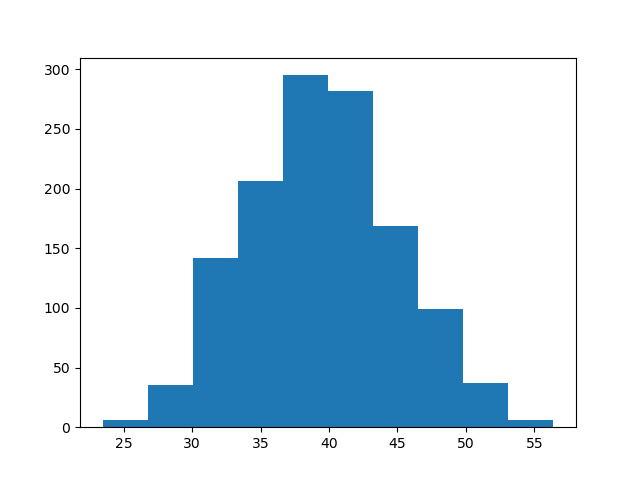
\includegraphics[scale=0.64]{histogram9.png}
\end{center}
\caption{Расподела допустивих решења тест примера \textit{ulaz9.txt}}
\label{hist9}
\end{figure}

\begin{table}[h!]
\begin{center}
\caption{\dvareda{Расподела потенцијалних решења тест\\ примера \textit{ulaz9.txt} према допустивости}}
\begin{tabular}{| c c c | c c |} \hline
Могућих & Допустивих & Удео & Најбоље & Средње\\ \hline
62.814 & 1277 & 2,03\% & 23,45 & 39,47\\ \hline
\end{tabular}
\label{udeo9}
\end{center}
\end{table}

Исто је у скрипту \textit{rando.py} урађено са још шест насумично генерисаних скупова од шест до осам тачака. Њихови резултати дати су на хистограму \ref{histrand} и у табели \ref{udeorand}, а веома личе на претходно добијене, уз напомену да је са порастом димензије проблема приметно смањење удела допустивих решења. Осетно је и повећање одступања средње вредности од минималне са једног и по на два до четири пута, при чему расподела сада више личи на неку гама или експоненцијалну.

\begin{figure}[h!]
\begin{center}
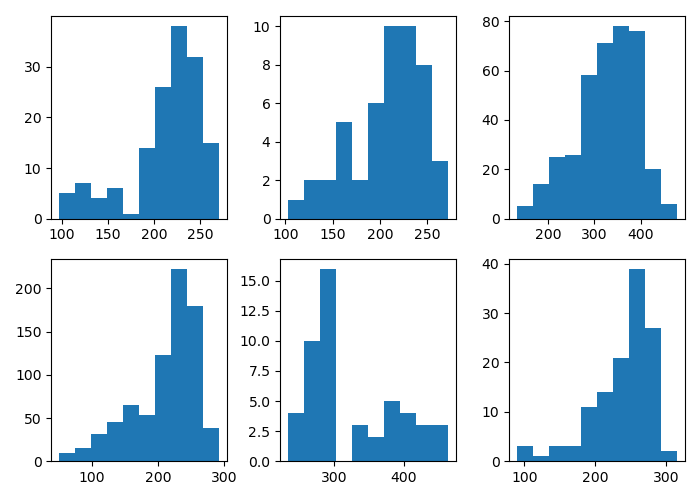
\includegraphics[scale=0.6]{histrandom.png}
\end{center}
\caption{Расподела допустивих решења случајних тест примера}
\label{histrand}
\end{figure}

\begin{table}[h!]
\begin{center}
\caption{\dvareda{Расподела потенцијалних решења случајних \\ тест примера према допустивости}}
\begin{tabular}{| c | c c c | c c |} \hline
& Могућих & Допустивих & Удео & Најбоље & Средње\\ \hline
\textit{r\string~1.txt} & 1172 & 148 & 12,6\% & 97,47 & 213\\
\textit{r\string~2.txt} & 197 & 49 & 24,9\% & 103,1 & 209\\
\textit{r\string~3.txt} & 8018 & 379 & 4,73\% & 133,9 & 328\\
\textit{r\string~4.txt} & 8018 & 784 & 9,78\% & 51,29 & 211\\
\textit{r\string~5.txt} & 1172 & 50 & 4,27\% & 233,8 & 326\\
\textit{r\string~6.txt} & 1172 & 124 & 10,6\% & 90,08 & 240\\ \hline
\end{tabular}
\label{udeorand}
\end{center}
\end{table}

У скриптовима \textit{histokazna.py} и \textit{randokazna.py} урађена је иста ствар, с тим што недопустива решења нису просто одбацивана већ су кажњавана према политици изложеној у првом делу поглавља. Резултати су исти; дакле, и даље се добијају тачна решења минимизацијом скора, што значи да је казна добро конципирана јер ниједна кажњена пермутација на крају није била боља од најбоље допустиве. Хистограми \textit{histokazna9.png} и \textit{historandokazna.png} изгледају очекивано -- имају изражене десне вредности -- тако да нису приказани у самом раду, али су сачувани и доступни читаоцу. И средње вредности су померене.

\subsection{Хеуристике}

Проблем многоугаоног раздвајања обрађен је у одређеној мери у литератури, мада углавном за верзију проблема која дозвољава да темена циљног полигона буду произвољна. Независно од дефиниције проблема, сва предложена решења досад су била \textbf{хеуристичке} природе, што подразумева \textit{усмерену претрагу} моделовану на основу особина проблема. Како су хеуристичка решења само приближна, овакви алгоритми углавном не дају тачно решење, али обично дају довољно добро у смислу прихватљивости за неке реалне потребе. Следе описи две главне хеуристике са гаранцијом квалитета, које се разликују управо по већ дискутованом домену темена циљног полигона.

Ситуација када темена могу бити произвољна дискутује се у углавном старијим радовима попут \cite{arora}. Новије тенденције подразумевају поделу простора неком сложенијом раздвајајућом структуром као што су кругови у \cite{cheung} или скупови правих у \cite{bonnet}. Дељена идеја набројаних радова заснована је на рекурзивној подели простора док се не дође до делова који садрже тачке само једне боје, а затим спајање тих делова у један. Прецизније, простор се дели на трапезе, који се даље деле на подтрапезе док није испуњен услов да се унутар њих налазе тачке само једне боје. Детаљи се могу погледати у изложеној литератури, али суштина је у свођењу полазног проблема на једноставнији, који се решава \textbf{динамичким програмирањем}. Заправо се углавном решавају два проблема -- налази се најмања многоугаона подела која садржи црвене тачке у унутрашњости и најмања многоугаона подела са плавим тачкама у унутрашњости -- након чега се одабира боље решење.

Временска сложеност таквог алгоритма, прецизно изложеног у раду \cite{mata}, износи $O(n^5)$, а фактор апроксимације је $O(\log k)$, где је $n$ број полазних тачака, а $k$ величина (број темена или страница) оптималног решења. Алтернативни алгоритам, који трапезе замењује правоугаоницима, сложености је $O(n^2)$, али са знатно већим апроксимационим фактором  $O(\log^3n)$. Приметити да се упрошћавањем партиционе структуре на правоугаонике не повећава само степен логаритма, већ и аргумент уместо величине оптималног решења постаје величина целог проблема, што није неочекивана цена значајног смањења временске сложености. Још бољи алгоритам предложен је у \cite{gud}, а извршава се у времену од $O(n\log n)$ и даје решење $O(\log k)$ горе од оптималног.

Алтернативни проблем, у ком се уместо обима минимизује број темена (тзв. комбинаторна сложеност) полигона, може се решити сличним алгоритмом изложеним у \cite{mitch}. Подела на трапезе извршава се у времену $O(n^8)$ са фактором апроксимације $O(\log k)$, а на правоугаонике у времену $O(n^2)$ са фактором $O(\log^2n)$.

Ситуација када су потенцијална темена фиксирана на задате скупове обојених тачака такође се дискутује у неколико радова. У њима се помињу и домени у којима решење овог проблема има реалну примену, као што су теорија класификације, рачунарски вид (енгл. \textit{computer vision}) и избегавање судара/колизија. Како је већ објашњено, управо ова верзија проблема проучавана је у овом раду. Наиме, полазна тачка овог рада \cite{csc} не говори ништа о домену темена, али фиксирање на задате тачке је природно решење за добијање коначног домена неопходног за касније изложени метахеуристички приступ.

Што се тиче цитата који следе, ипак постоји неколико разлика међу њима, као и у односу на поставку проблема у овом раду. Прва, ситна, јесте у томе што се у њима скупови не означавају као црвени и плави, већ унапред као спољашњи и унутрашњи, мада се то ограничење лако превазилази тако што се алгоритам покрене двапут, са различитим улогама црвеног и плавог скупа, а затим одабере боље решење у смислу скора. Друга, већа, јесте да се решавају само знатно олакшане верзије задатка, без задирања у пуну општост проблема.

Рад \cite{eades} ограничава се на случај када скуп унутрашњих гради конвексан многоугао односно једнак је свом конвексном омотачу. У том случају се у времену $O(n\log n)$ може добити приближно решење са константним фактором апроксимације, највише дупло већег обима од оптималног. Детаљан поступак доступан је у раду, а укратко: састоји се из формирања конвексног полигона од унутрашњих тачака, затим формирања конвексног полигона од спољашњих тачака садржаних у првом конвексном омоту и једне заједничке странице, и напослетку „исецања“ другог скупа из првог.

Рад \cite{edels} ограничава се на случајеве када се претражују искључиво конвексни полигони, с тим што су за разлику од првог рада дозвољена и решења која укључују спољашње тачке. То је, ипак, и даље знатно ужи скуп од свих простих многоуглова, при чему такође постоји разлика у томе што се не минимизује обим, већ величина решења (број темена односно страница). И ту је временска сложеност $O(n\log n)$ односно $O(nk)$ (изложена су два алгоритма), мада је погодност то што је први оптималан -- проналази тачно решење -- док други греши тако што у решење укључи највише једну тачку више него што је потребно, што није превелика грешка.

\section{Метахеуристике}

Како се испоставило да до тренутка писања овог рада није било успешних покушаја решавања задатог проблема у својој пуној општости, разумно решење доноси прибегавање \textbf{метахеуристикама} као општим стратегијама претраге за решавање оптимизационих проблема. Иако је свака формулисана независно од конкретног проблема, свака је на свој начин прилагодљива посебном проблему који се решава, па тако и минималном полигоналном раздвајању два скупа тачака.

\subsection{Случајна претрага}

Алгоритам \textbf{случајне претраге} представља најпростију метахеуристичку методу. Састоји се из генерисања одређеног броја насумичних решења и простог одређивања најбољег у смислу скора. Управо ово урађено је у скрипту \textit{algoritmi.py}, при чему је за већ познате тест примере направљено по петсто различитих јединки, након чега је одабрана најбоља. Како би експеримент био поновљив, фиксирано је семе генератора псеудослучајних бројева, мада је за потребе провере опробано и неколико независних покретања без фиксирања. Упоредни резултати дати су у табели \ref{slucajna}. Отприлике је за половину примера погођено оптимално решење, док у осталима постоји варирајућа релативна, али углавном не превелика апсолутна грешка решења.

\begin{table}[h!]
\begin{center}
\caption{Поређење исцрпне са резултатима случајне претраге}
\begin{tabular}{| c | c c | c c |} \hline
& Исцрпна & Случајна & Рел. гр. & $\delta$\\ \hline
\textit{ulaz9.txt} & 23,45 &  27,95 & 19,2\% & 3\\
\textit{random1.txt} & 97,47 &  97,47 & 0,00\% & 0\\
\textit{random2.txt} & 103,1 &  103,1 & 0,00\% & 0\\
\textit{random3.txt} & 133,9 & 256,9 & 91,9\% & 3\\
\textit{random4.txt} & 51,29 & 108,1 & 111\% & 3\\
\textit{random5.txt} & 233,8 & 233,8 & 0,00\% & 0\\
\textit{random6.txt} & 90,08 & 93,99 & 4,34\% & 1\\ \hline
\end{tabular}
\label{slucajna}
\end{center}
\end{table}

Апсолутна и релативна грешка ипак нису најбоље мерило успешности када се примењују на скорове постигнуте метахеуристичким алгоритмима. Најчешће је прикладније непосредно поредити јединке односно на неки начин исказати сличност у коду решења (генетску сличност) уместо у постигнутом скору. Тако се конкретније види колико је разматрана јединка близу оптималној, јер је понекад једна промена у коду довољна да можда чак и недопустиво решење (бесконачна грешка) доведе до оптимума, док су нека по скору блиска оптималном (мала апсолутна и релативна грешка) малтене непоправљива. Како су кодови углавном низови, примењују се разне векторске мере различитости, попут Хаминговог или растојања Минковског.

У простору пермутација прича је мало другачија, поготову у случајевима попут представљања многоуглова, где су нпр. троуглови $ABC$ и $BCA$ (други је лева ротација првог за једно место) или $ABC$ и $CBA$ (други је инверзија првог) једнаки. За потребе мерења растојања између оваквих структура, имплементиран је алгоритам заснован на \textbf{Левенштајновом растојању}, типу растојања уређивања (енгл. \textit{edit distance}), а чији су резултати у табели представљени грчким словом $\delta$. Ови бројеви представљају најмањи број измена које је потребно начинити да би се добијени многоугао свео на оптимални, при чему су дозвољени замена елемената (обострана, нпр. замена $0 \leftrightarrow 1$ од ниске $03251$ прави $13250$, не недопустиво $13251$), њихово додавање или избацивање. У питању је подскуп мутација (о њима ће касније бити речи), погодно одабран тако да је динамичким програмирањем могуће егзактно минимизовати број неопходних замена у полиномском времену уместо у неприхватљивом експоненцијалном. На конкретном примеру случајне претраге, приметно је да су сва добијена решења врло блиска најбољем, чак и са релативном грешком преко 100\%.

\subsection{Локална претрага}

Још један једноставнији пример метахеуристика представља \textbf{локална претрага}. Овај алгоритам карактерише постепено унапређивање почетног решења, које је углавном насумично генерисано. У сваком кораку (итерацији) разматра се решење у околини тренутног и оно замењује тренутно уколико му је прилагођеност већа. Сигнал за крај алгоритма је испуњавање неког критеријума заустављања, што је углавном достигнут фиксирани број итерација, а алтернативно максималан број итерација без замена текућег решења (конвергенција) или чак укупно време извршавања, уколико је то применљиво.

Пре имплементације, уз претходно дефинисану процедуру \textbf{генерисања случајне јединке}, неопходно је дефинисати околину тј. суседство сваке јединке. Како се у даљем раду планира конструкција генетског алгоритма, ово је учињено помоћу \textbf{оператора мутације}, који има исту семантику -- њиме се добијају решења довољно слична полазном, што је карактеристика и суседства. Конкретно, имплементирано је седам видова мутација, четири својствене пермутацијским проблемима -- уметање, замена, обртање (инверзија), мешање -- две карактеристичне за проблеме са кодовима променљиве дужине -- додавање и одузимање -- и једна уобичајена промена вредности. Који ће тачно бити примењен, зависи од случајног избора у току извршавања, уз два важна ограничења: за троуглове (кодове дужине три) искључиво имају смисла додавање и случајна промена, док су за $n$-тоуглове (кодове максималне дужине) једино те две операције неизводљиве.

Имплементирана је и напреднија верзија локалне претраге позната као \textbf{симулирано каљење}. Свој назив дугује процесу каљења челика, чији је циљ повећање чврстине метала. Челик се загрева до одређене температуре, након чега се постепено хлади, пошто би нагло хлађење довело до пуцања. Ово је пресликано у оптимизациони алгоритам на следећи начин: у кораку замене текућег решења новим, са одређеном вероватноћом која опада кроз време, могуће је прихватити ново које није боље од старог. На тај начин се смањује вероватноћа превремене конвергенције ка локалном оптимуму који није и глобални. Притом се све време чува дотад најбоље пронађено решење, тако да оно не бива изгубљено чак и ако претрага заврши на лошем правцу.

Упоредни резултати примене алгоритама локалне претраге дати су у табели \ref{lokalna}. И овога пута, иницијализован је генератор псеудослучајних бројева, уз претходне провере да све ради и без тога. Примена се налази у скрипту \textit{algoritmi.py}. Почевши од махом недопустивих решења (бесконачан скор), други приступ је у петсто итерација углавном налазио глобалне оптимуме, док се први заглављивао. Још једном је похвално то што су растојања уређивања прилично ниска, а поготову то што једино непогођено решење код симулираног каљења од оптимума дели само једна замена, мада је и без ње скор веома близак.

\begin{table}[h!]
\begin{center}
\caption{Поређење исцрпне са резултатима локалне претраге}
\begin{tabular}{| c | c | c c | c c |} \hline
& Исцрпна & Локална & $\delta$ & Сим. кал. & $\delta$\\ \hline
\textit{ulaz9.txt} & 23,45 & 27,86 & 4 & 23,68 & 1\\
\textit{random1.txt} & 97,47 & 97,47 & 0 & 97,47 & 0\\
\textit{random2.txt} & 103,1 & 103,1 & 0 & 103,1 & 0\\
\textit{random3.txt} & 133,9 & 133,9 & 0 & 133,9 & 0\\
\textit{random4.txt} & 51,29 & 51,29 & 0 & 51,29 & 0\\
\textit{random5.txt} & 233,8 & 256,5 & 4 & 233,8 & 0\\
\textit{random6.txt} & 90,08 & 226,3 & 3 & 90,08 & 0\\ \hline
\end{tabular}
\label{lokalna}
\end{center}
\end{table}

Још сложеније алтернативе претходно изложених приступа јесу \textbf{итеративна локална претрага} и \textbf{метода променљивих околина}. У првој, покушај избегавања локалног минимума огледа се у узастопној примени локалне претраге над различитим почетним јединкама, за које углавном постоји услов да нису довољно сличне. Примера ради, за проблем са $n$ улазних тачака могле би се покренути $n-2$ локалне претраге за почетна решења дужине $3$ до $n$. У другој, простор претраге дели се на околине које се независно претражују. И овде би околине могле бити дефинисане као решења неке фиксне дужине. Трећа алтернативна могла би бити \textbf{табу претрага}, која оперише над суженим суседством, избегавајући решења из скупа забрањених потеза. Тај скуп чине јединке које се у претходним корацима нису показале као обећавајуће, чиме је јасно да су лош избор. Ипак, услед задовољавајуће успешности првих приступа, други нису имплементирани.

\subsection{Генетски алгоритам}

Претходно разматрани алгоритми припадали су групи \textbf{метахеуристика заснованих на унапређењу једног решења} (скраћено \textit{S-метахеуристике}). Сваки приступ тог типа започињао је једним решењем које се у сваком кораку претраге углавном побољшавало заменом са неким бољим оближњим решењем. Може се рећи да се јединка кретала кроз простор, тако да се ове технике називају и \textit{метахеуристике засноване на путањи}. Други приступ чине \textbf{метахеуристике засноване на популацији јединки} (\textit{P-метахеуристике}), које се сатоје од углавном случајног генерисања почетне популације, а затим итеративног унапређивања исте. Најпознатији пример ове групе метахеуристичких алгоритама јесу \textbf{еволутивна израчунавања}, са генетским алгоритмом као најистакнутијим представником.

\textbf{Генетски алгоритам} заснован је на \textit{теорији еволуције}, према којој углавном опстају само најбоље прилагођене јединке (хромозоми, низови гена). Решења из почетне популације (генерације) укрштају се, а њихови потомци, уз евентуалне мутације појединих гена, улазе у састав наредне генерације. Дакле, на почетку се случајно направи полазна генерација и евалуира јој се прилагођеност. Потом се, док није испуњен услов заустављања, ради следеће: одаберу се јединке из текуће популације над којима се примењују генетски оператори, укрштају се изабране јединке, потомци евентуално мутирају, нова популација се евалуира и постаје текућа. \textbf{Теорема о схемама} осигурава да се, уз погодно подешене параметре, сменом генерација континуирано добија нова популација која је боље прилагођена окружењу од претходне.

Када је у питању конкретан проблем који се решава, већина корака алгоритма већ је дефинисана: репрезентација (кодирање) решења, функција прилагођености (погодности, циља -- овде се поистовећују), случајно генерисање иницијалне популације. Критеријум заустављања је достигнут максималан број итерација. Унапред је имплементиран и један генетски оператор -- мутација. У склоп јединке додата је једино реализација \textbf{оператора селекције} (случајна, турнирска, рулетска и ранговска) и \textbf{укрштања} (својствено пермутацијама -- првог реда, позиционо и размештање ивица). Сам алгоритам примењен је у скрипту \textit{algoritmi.py}, при чему је коришћен и принцип \textit{елитизма}.

У циљу побољшања квалитета коначног решења, имплементирана је заправо \textbf{хибридизација} генетског алгоритма са симулираним каљењем. Оно се у свакој итерацији примењује на најбољу јединку текуће генерације. Алтернативно, могло се примењивати и на неколико најприлагођенијих јединки, неколико насумичних или чак на све. Још једна могућности била је прављење почетне генерације од каљених јединки или хибридизација са другом погодном S-метахеуристиком, али и \textit{еволуција параметара} или \textit{паралелизација алгоритма}.

\begin{table}[h!]
\begin{center}
\caption{Поређење претходних са резултатима генетског алгоритма}
\begin{tabular}{| c | c | c c c | c c |} \hline
& Исцрпна & Сл. $\delta$ & Лок. $\delta$ & Сим. $\delta$ & Ген. & $\delta$\\ \hline
\textit{ulaz9.txt} & 23,45 & 3 & 4 & 1 & 23,45 & 0\\
\textit{r\string~1.txt} & 97,47 & 0 & 0 & 0 & 97,47 & 0\\
\textit{r\string~2.txt} & 103,1 & 0 & 0 & 0 & 103,1 & 0\\
\textit{r\string~3.txt} & 133,9 & 3 & 0 & 0 & 133,9 & 0\\
\textit{r\string~4.txt} & 51,29 & 3 & 0 & 0 & 51,29 & 0\\
\textit{r\string~5.txt} & 233,8 & 0 & 4 & 0 & 233,8 & 0\\
\textit{r\string~6.txt} & 90,08 & 1 & 3 & 0 & 90,08 & 0\\ \hline
\end{tabular}
\label{genetski}
\end{center}
\end{table}

Поређење са претходним алгоритмима приказано је у табели \ref{genetski}. Параметри попут величине популације и броја итерација подешени су тако да је поређење фер -- око петсто евалуација функције погодности. Како је и очекивано, у складу са тиме да је генетски алгоритам један од оних од којих се иначе највише очекује и који иначе даје најбоље резултате од свих досад изложених, и овде се одлично показао, са свим погођеним глобалним оптимумима. У овом алгоритму је, иначе, први пут коришћено рачунање скора са казном, како би се разликовале боље недопустиве јединке од лошијих, што је битан детаљ приликом свих типова селекције, а поготову рулетске, која и није дефинисана за бесконачне скорове. Опробана је и верзија без казне (ручна еволуција параметара алгоритма), али се она показала као мање погодна.

Важно је напоменути и да је природа проблема таква да су сви добијени резултати, чак и кад нису оптимални, врло блиски најбољем према дефинисаној мери растојања уређивања. То значи да добијену јединку од оптималне дели само неколико простих мутација -- замене, уметања, брисања. У складу са тим, резултати генетског алгоритма су побољшани хибридизацијом, пошто унапређивање решења смањује потребу за такозваном „срећном мутацијом“, која је често неопходна код примене популацијских приступа на овакве проблеме. Из истог разлога је подешена релативно висока стопа мутације -- чак 30\%.

\subsection{Јато птица}

Размотрене су и могућности \textbf{оптимизације ројем честица}. Овај приступ је заснован на интелигенцији ројева, која се огледа у сложеном социјалном понашању појединачних јединки унутар групе попут јата птица, колоније пчела или мрава. Примера ради, када рој (назив за популацију код оваквих алгоритама) тражи храну, честица (назив за јединку код оваквих алгоритама) која је најуспешнија у потрази (најближа храни) на неки начин привлачи остатак групе. Поред тога, свака честица прати и сопствени инстинкт у претрази, чиме се смањује могућност заглављивања у локалном оптимуму ка којем може вући најбоља јединка у неком тренутку. Другим речима, у оптимизациони процес пресликава се физичко кретање јединки кроз простор.

Конкретно је имплементирана верзија проблема позната као \textbf{оптимизација јатом птица}. При овом приступу, свака честица усмерава се на основу своје тренутне позиције, своје дотад најбоље позиције, као и дотад најбоље позиције на нивоу читаве популације. Ово се укруг понавља све док није задовољен критеријум заустављања, попут достигнутог прописаног броја итерација, при чему се у свакој итерацији ажурирају најбоље вредности решења за сваку честицу, као и за рој у целини. Како се ажурирање своди на рачунање растојања између честица, израчунавање брзина и њихово додавање честицама, тако сложене односе није лако моделовати у нестандардним просторима, где спада и простор пермутација, у ком је изучавани проблем.

Наизглед добро замишљен модел, који је послужио као идејна основа овдашње имплементације, изнет је у \cite{clerc}, а први корак у његовој реализацији већ је начињен дефиницијом растојања односно реконструкцијом пута (низа измена) између јединки. Наиме, аутор цитираног рада предлаже редефиницију круцијалних оператора на следећи начин -- \textbf{одузимањем честица} добија се низ транспозиција који другу преводи у прву (растојање), \textbf{брзине} су низови транспозиција и њихово \textbf{сабирање} заправо је конкатенација, \textbf{множење брзине} заправо је продужавање (или скраћивање) низа транспозиција, док је \textbf{додавање брзине честици} примена низа транспозиција на њу.

Осим транспозиција (замена елемената), у овом раду је дозвољено и додавање и брисање тачака, како би се решио проблем пермутација различитих дужина. Сама реконструкција пута, како је већ напоменуто, заснована је на Левенштајновом растојању и раније је реализована. Без проблема су реализовани и остали оператори, при чему је у скрипту \textit{jedinka.py} имплементирана нова класа за представљање низа измена. Са апсолутно истим образложењем као код претходног описа генетског алгоритма, имплементирана је заправо хибридизација оптимизације јатом птица са симулираним каљењем, што значи да је на крају сваке итерације мало побољшавано глобално најбоље решење. И овде су параметри подешени на фер начин према осталим приступима. Примена је доступна у скрипту \textit{algoritmi.py}, а добијени резултати, који су иначе веома задовољавајући, представљени су у табели \ref{jato}.

\begin{table}[h!]
\begin{center}
\caption{Поређење претходних са резултатима јата птица}
\begin{tabular}{| c | c | c | c c |} \hline
& Исцрпна & Претходно $\delta$ & Јато & $\delta$\\ \hline
\textit{ulaz9.txt} & 23,45 & \{3, 4, 1, 0\} & 222,5 & 1\\
\textit{r\string~1.txt} & 97,47 & \{0, 0, 0, 0\} & 97,47 & 0\\
\textit{r\string~2.txt} & 103,1 & \{0, 0, 0, 0\} & 103,1 & 0\\
\textit{r\string~3.txt} & 133,9 & \{3, 0, 0, 0\} & 133,9 & 0\\
\textit{r\string~4.txt} & 51,29 & \{3, 0, 0, 0\} & 51,29 & 0\\
\textit{r\string~5.txt} & 233,8 & \{0, 4, 0, 0\} & 233,8 & 0\\
\textit{r\string~6.txt} & 90,08 & \{1, 3, 0, 0\} & 90,08 & 0\\ \hline
\end{tabular}
\label{jato}
\end{center}
\end{table}

\section{Велики пример}

За крај, спроведен је \textbf{експеримент} над великим случајно генерисаним тест примером од чак тридесет униформно расподељених тачака на мрежи димензија $1000 \times 1000$ тј. у области $[1, 1000] \times [1, 1000]$ равни. Подсећања ради, у питању је огроман простор претраге од чак $\frac{1}{2} \sum_{k=3}^{30} {30 \choose k} (k-1)! \approx 10^{31}$ различитих многоуглова. Пример је као \textit{ulaz30.txt} генерисан у скрипту \textit{veliki.py}, у ком је и испитан. Пуштени су сви имплементирани метахеуристички алгоритми, поново уз пажњу да је поређење \textbf{фер} -- овога пута по око сто хиљада евалуација функције погодности. Упоредни резултати дати су у табели \ref{veliki}, док је графички приказ добијених решења дат на слици \ref{poredjenje30}, као и у датотеци \textit{skor30.txt}, која сведочи о приличној различитости добијених кодова.

\begin{table}[h!]
\begin{center}
\caption{Поређење на великом тест примеру}
\begin{tabular}{| c | c c c c c |} \hline
& Случ. & Локална & Сим. кал. & Ген. алг. & Јато\\ \hline
\textit{ulaz30.txt} & $\infty$ & 4588,71 & 3732,68 & 3831,71 & 4908,34\\ \hline
\end{tabular}
\label{veliki}
\end{center}
\end{table}

\begin{figure}[h!]
\begin{center}
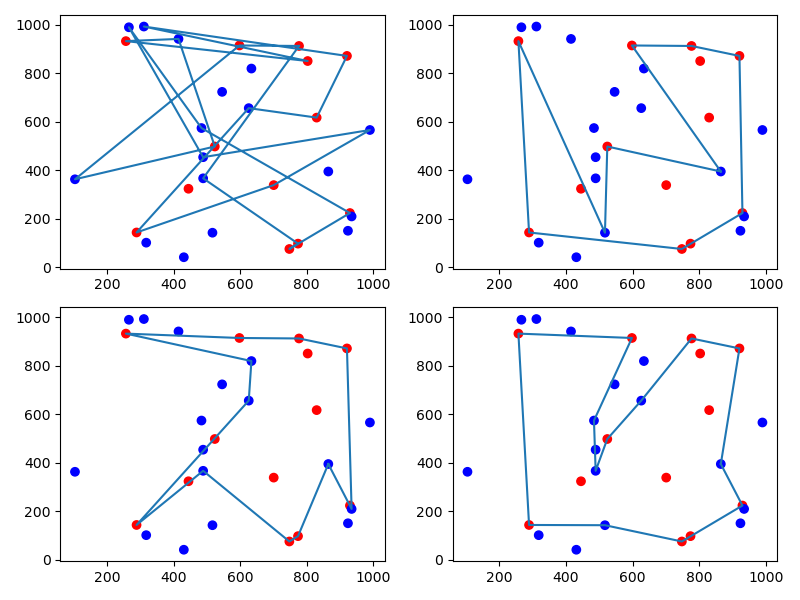
\includegraphics[scale=0.6]{poredjenje30.png}
\end{center}
\caption{Поређење на великом тест примеру}
\label{poredjenje30}
\end{figure}

Како је донекле и очекивано, случајна претрага (горње десно) није се снашла у несистематичном прегледању незнатног дела (само $10^{-24}\%$) простора претраге, тако да је коначно решење прилично недопустиво: у питању је велики многоугао пун самопресека. Остале методе дале су пристојна решења -- редом локална претрага (средње лево), симулирано каљење (средње десно), генетски алгоритам (доње лево) и оптимизација јатом птица (доње десно) -- при чему је претрага сваког метода завршила у другом делу простора. Наиме, разлика уређивања између те четири пермутације је пет до девет, што није премало, док је разлика између њих и недопустиве добијене случајном претрагом петнаест или шеснаест, што је већ превелик број замена. Поређења ради, на графику је дат и чист приказ задатог проблема (горње лево).

Анегдотално, симулирано каљење је у овом примеру однело победу када је у питању скор решења, али уз неколико узастопних покретања са различитих семенима генератора псеудослучајних бројева утврђено је да то није чврсто правило, већ склоп случајности. Ипак, увек су блиска решења; испоставља се да само каљење може да парира генетском алгоритму, за разлику од једноставне локалне претраге која најчешће буде лошија, иако и она некад надмаши друге приступе. Оптимизација јатом птица је, независно од параметара, подбацила, чак и након што јој је дозвољено да буде у предности тиме што више пута евалуира функцију прилагођености од предвиђених сто хиљада.

Када је у питању \textbf{експериментално окружење}, хардверске карактеристике су следеће -- четворојезгарни процесор \textit{AMD Ryzen 5 3550H (with Radeon Vega Mobile Gfx)} радног такта 2,10 GHz са примарном интегрисаном графичком картицом \textit{AMD Radeon Vega 8 Graphics}, радна меморија од 12 GB (од чега је 2 GB резервисано за интегрисану графику) типа \textit{DDR4}, као и веома брза и код улазно-излазних операција ефикасна \textit{SSD} трајна меморија од 512 GB типа \textit{PCIe NVMe}. Доступна је и секундарна независна графичка картица \textit{Radeon RX 560X Series} са 4 GB виртуелне радне меморије, али није коришћена у израчунавањима. Оперативни систем је лиценцирани 64-битни и у потпуности ажурни \textit{Windows 10 Pro}. Програмски језик имплементације је релативно ажурни \textit{Python 3.7.6} (не користе се новије верзије зарад компатибилности са свим неопходним библиотекама), интерпретиран званичним минималистичким развојним окружењем \textit{IDLE}. Пун податак о компилацији је \textit{[MSC v.1916 64 bit (AMD64)] on win32}. Списак коришћених екстерних модула и њихових тачних верзија дат је у уобичајеној датотеци са зависностима пригодно названој \textit{reqs.txt}.

\section{Закључак}

Минимално многоугаоно раздвајање два скупа тачака у равни до овог тренутка је био прилично неистражен проблем. Иако су се многи аутори бавили сличним задацима, решаван је или хеуристички нападљив измењени проблем са дозвољеним произвољним тачкама унутар решења или исто хеуристички нападљиве олакшане верзије попут оних када је један од скупова конвексан или обухвата други скуп.

Из тог разлога је, у сврхе превазилажења досадашњег недостатка макар приближног решења проблема у својој пуној општости, у овом раду имплементирано неколико различитих метахеуристичких алгоритама, са задовољавајућим резултатима. Као најбољи показао се генетски алгоритам, заснован на унапређивању популације јединки, уз погодну хибридизацију са симулираним каљењем, приступом заснованим на итеративном побољшању једног решења. То је и очекивано када се примети генетска блискост свих добијених јединки са оптималним. Ипак, у неколико случајева ни само симулирано каљење није много заостајало. Могућа примена решења могла би се наћи у теорији класификације, рачунарском виду или избегавању судара/колизија.

Даља истраживања могла би се фокусирати на алгоритме који нису детаљно проучени у овом раду. Из групе S-метахеуристика могли би се издвојити итеративна локална претрага, метод променљивих околина или пак табу претрага. Из групе P-метахеуристика, то би могла бити оптимизација другим ројевима честица попут колонија пчела или мрава или чак неки напредни меметски алгоритам. Пажња би се могла посветити и еволуцији параметара алгоритама, као и паралелним верзијама сваког приступа, од чега је могуће да би дистрибуирани острвски генетски алгоритам ефектно дао решење проблема.

\newpage
\addcontentsline{toc}{section}{Литература}
\appendix
\bibliography{Minima\string~1}
\bibliographystyle{apalike}

\end{document}
